\section{Evaluation}
In order to evaluate the usefulness of exploration in AWA$^*$ a number of experiments were conducted on the sliding tile puzzle. All experiments are run on an 8-core 1.70GHz machine with 16 gigabytes of memory. For all experiments, the two exploration techniques will be compared to a standard AWA$^*$ implementation which will serve as the benchmark. One hundred instances of the unit cost 12-puzzle were used to compare the three algorithms.

The primary focus was on the Unit Cost Sliding Tile puzzle using the Manhattan Distance Heuristic. Various weights are used across the three algorithms and two different values of $\epsilon$, $0.1$ and $0.3$ \cite{valenzano2014comparison}, are used for $\epsilon-$AWA$^*$ and $\alpha \beta-$AWA$^*$. Depending on the value of $\epsilon$, $\epsilon-$AWA$^*$ and $\alpha \beta-$AWA$^*$ will be abbreviated to $0.1$-$\epsilon$, $0.3$-$\epsilon$, $0.1$-$\alpha \beta$, and $0.3$-$\alpha \beta$ respectively. The beta distribution in all $\alpha \beta-$AWA$^*$ instances is fixed at $\alpha=5$ and $\beta=0.6$.

There are also two small extensions. In the first, the Inverse Sliding Tile Puzzle is briefly investigated using the Manhattan Distance Heuristic. In these experiments, the value of $\epsilon$ is fixed at 0.3, and only 3 weights are considered: 1.3, 5, and 10. The Inverse Sliding Tile Puzzle was chosen because it tends to be harder than the Unit Cost variant. The second extension involves degrading the heuristic and using the Correct Tile Placement Heuristic. This was done to investigate how exploration may help or hinder with a highly uninformed heuristic.

\subsection{Unit Cost Tile Puzzle}
In general, it was found that adding exploration to AWA* for the sliding tile puzzle proved to be very effective. Both $\epsilon-$AWA$^*$ and $\alpha \beta-$AWA$^*$ required fewer incumbent solutions to zero in on the optimal solution, as summarized in Table \ref{tad:num-sol}.

\begin{table}
\def\arraystretch{1.3}
\begin{tabular}{ |c||c|c|c|c|c|  }
    \hline
    \multicolumn{6}{|c|}{Average Number of Incumbent Solutions} \\
    \hline
    Weight& AWA* & $0.1$-$\epsilon$ &$0.3$-$\epsilon$&$0.1$-$\alpha \beta$ & $0.3$-$\alpha \beta$\\
    \hline
    1.3 & \textbf{2.24} & 2.25 & 2.28 & 2.26 & 2.28\\
    \hline
    2 & 3.91 & 4.09 & \textbf{3.75} & 3.94 & 3.86\\
    \hline
    3 & 7.07 & 6.69 & \textbf{6.07} & 6.54 & 6.19\\
    \hline
    5 & 11.15 & 10.37 & \textbf{9.28} & 10.05 & 9.65\\
    \hline
    10& 15.49 & 15.03 & \textbf{13.27} & 14.56 & 13.74\\
    \hline
\end{tabular}
\caption{Incumbent Solutions}\label{tad:num-sol}
\end{table}

In all cases, except for weight=1.3, $0.1$-$\epsilon-$AWA$^*$ required the fewest incumbent solutions before finding the optimal. However, both exploration were consistently better than standard AWA* by this metric. 

To gauge the complexity of each algorithm the number expanded nodes and the total number of generated nodes are considered. By this metric exploration shows a huge improvement over standard AWA*, as shown in Figure \ref{fig:nodes}.

\begin{figure}
    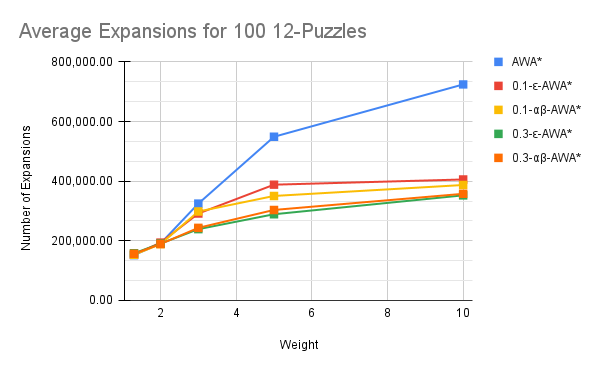
\includegraphics[width=\linewidth]{media/Average Expansions for 100 12-Puzzles.png}
    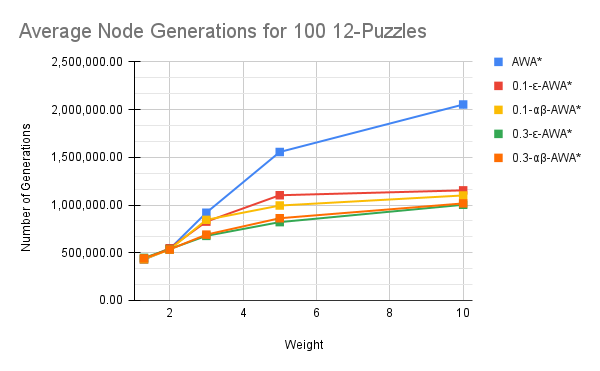
\includegraphics[width=\linewidth]{media/Average Node Generations for 100 12-Puzzles.png}
    \caption{Complexity with Manhattan Distance Heuristic.} \label{fig:nodes}
\end{figure}

Standard AWA* requires close to 800,000 expansions in the case of a weight of 10, while all four exploration algorithms require in the neighbourhood of 400,000. AWA* seems to be far more impacted by increasing the weight, and thereby degrading the accuracy of the evaluation function, than the $\epsilon$ and $\alpha\beta$ variants--which both require a similar number of expansions for a weight of 5 and a weight of 10. Perhaps most surprising is that setting $\epsilon$ to 0.3 gets the best results.

Adding to this, exploration in anytime sees an analogous improvement in its runtime when compared to standard AWA*, as seen in Figure \ref{fig:run}. This is not guaranteed as it could be the case that the improved node selection procedure takes enough time so as to offset the time savings of expanding fewer nodes. In the cases of $\epsilon-$AWA$^*$ and $\alpha \beta-$AWA$^*$, the node selection procedure is sufficiently simple that the expansion savings result in (proportionally) equal time savings. 

\begin{figure}
    \begin{center}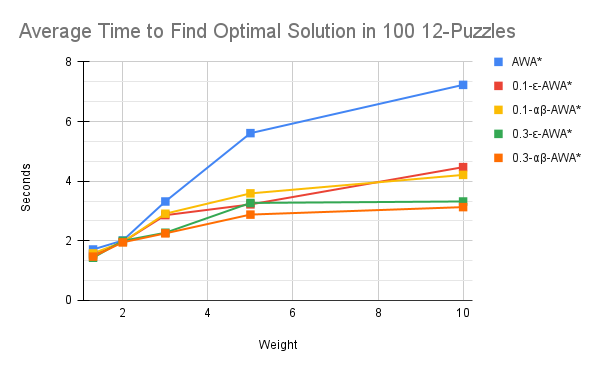
\includegraphics[scale=0.35]{media/Average Time to Find Optimal Solution in 100 12-Puzzles.png}\end{center}
    \caption{Average Time to Find Optimal Solution}\label{fig:run}
\end{figure}

To summarize the above results, it's useful to look at how quickly each algorithm converges on the optimal solution over time and over number of expansions. Given both the $\epsilon$ and $\alpha\beta$ variants required fewer incumbent solutions, fewer expansions to get those solutions, and took less time, it should be the case that they approach the optimal solution much faster than AWA*, which is precisely what we see in Figure \ref{fig:conv-man}.

\begin{figure}
    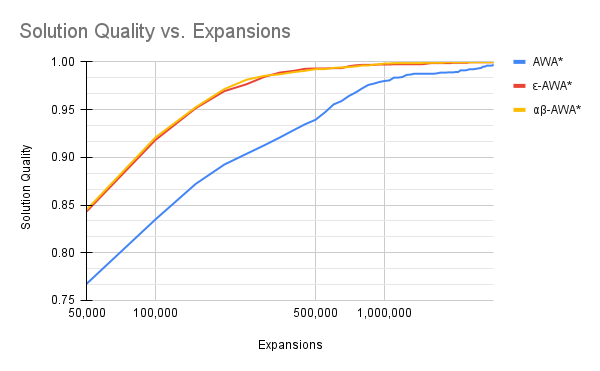
\includegraphics[width=\linewidth]{media/man-Solution Quality vs. Expansions.png}
    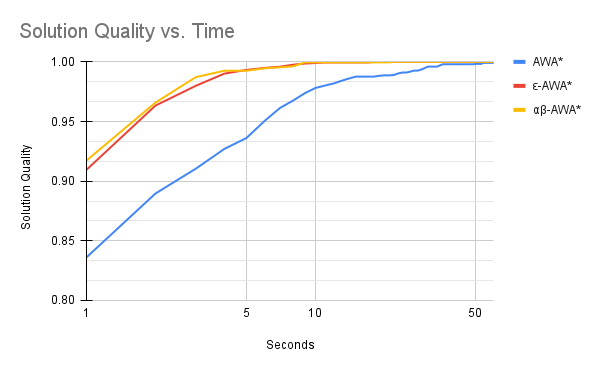
\includegraphics[width=\linewidth]{media/man-Solution Quality vs. Time.png}
    \caption{Quality Convergence with Manhattan Distance Heuristic.} \label{fig:conv-man}
\end{figure}

Here, solution quality is $\frac{incumbent-cost}{optimal-cost}$ for a given problem and the solution qualities are averaged across all problem instances. For expansion convergence, the incumbent cost was polled every 50,000 expansions; for the time convergence the incumbent cost was polled every one second (notice the log x-axis in both charts). In this, only a weight of 10 and an epsilon value of 0.3 were considered. 

\subsection{Inverse Cost Tile Puzzle}

\begin{table}
\def\arraystretch{1.3}
\begin{tabular}{ |c||c|c|c|  }
    \hline
    \multicolumn{4}{|c|}{Average Number of Incumbent Solutions} \\
    \hline
    Weight& AWA* & $0.3$-$\epsilon$-AWA$^*$ & $0.3$-$\alpha\beta$-AWA$^*$\\
    \hline
    1.3 & 3.14 & 3.13 & \textbf{2.97} \\
    \hline
    5 & 21.91 & 15.66 & \textbf{15.41} \\
    \hline
    10& 30.8 & \textbf{20.4} & 21.26 \\
    \hline
\end{tabular}
\caption{Incumbent Solutions}\label{tab:inv-sol}
\end{table}

\begin{table}
\def\arraystretch{1.3}
\begin{tabular}{ |c||c|c|c|  }
    \hline
    \multicolumn{4}{|c|}{Average Number of Seconds to Find Optimal} \\
    \hline
    Weight& AWA* & $0.3$-$\epsilon$-AWA$^*$ & $0.3$-$\alpha\beta$-AWA$^*$\\
    \hline
    1.3 & 2.25 & \textbf{2.15} & \textbf{2.15} \\
    \hline
    5 & 16.38 & 6.65 & \textbf{6.34} \\
    \hline
    10& 21.57 & \textbf{7.3} & 8.09 \\
    \hline
\end{tabular}
\caption{Runtime}\label{tab:inv-avg-time}
\end{table}

\begin{table}
\def\arraystretch{1.3}
\begin{tabular}{ |c||c|c|c|  }
    \hline
    \multicolumn{4}{|c|}{Average Number of Expansions} \\
    \hline
    Weight& AWA* & $0.3$-$\epsilon$-AWA$^*$ & $0.3$-$\alpha\beta$-AWA$^*$\\
    \hline
    1.3 & \textbf{186,038.15} & 211,198.92 & 206,175.07 \\
    \hline
    5 & 1,408,646.74 & 622,837.79 & \textbf{587,692.64} \\
    \hline
    10& 1,901,236.58 & \textbf{709,049.28} & 769,546.95 \\
    \hline
\end{tabular}
\caption{Expansions}\label{tab:inv-avg-exp}
\end{table}

\begin{table}
\def\arraystretch{1.3}
\begin{tabular}{ |c||c|c|c|  }
    \hline
    \multicolumn{4}{|c|}{Average Number of Node Generations} \\
    \hline
    Weight& AWA* & $0.3$-$\epsilon$-AWA$^*$ & $0.3$-$\alpha\beta$-AWA$^*$\\
    \hline
    1.3 & \textbf{529,095.35} & 603,706.60 & 589,437.60 \\
    \hline
    5 & 4,003,219.50 & 1,780,788.61 & \textbf{1,680,521.61} \\
    \hline
    10& 5,401,559.63 & \textbf{2,027,138.81} & 2,200,575.94 \\
    \hline
\end{tabular}
\caption{Generations}\label{tab:inv-avg-gen}
\end{table}

\subsection{Degraded Heuristic in Unit Cost Sliding Tiles}
Given the promising results above, it would be expected that when the heuristic gets degraded, exploration should help even more as degraded heuristics result in more plateaus and less confidence about the `best' node in the open list. However, in looking at the summary evaluation of solution quality over time and expansions using the Correct Tile Placement heuristic, this did not turn out to be case, as seen in Figure \ref{fig:conv-correct}.

Here, again, only a weight of 10 and an epsilon value of 0.3 were considered. For expansions, each algorithm was limited to 3,000,000 expansions, and for time each algorithm was limited to one minute. 

\begin{figure}
    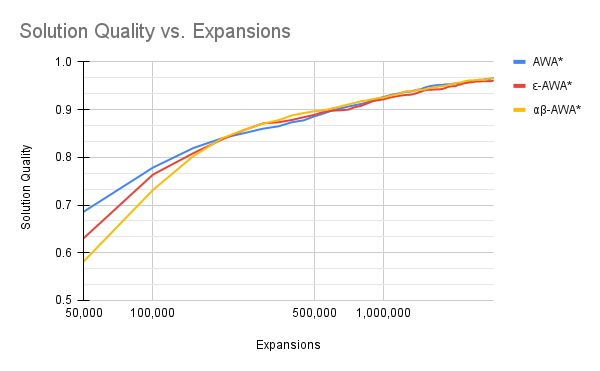
\includegraphics[width=\linewidth]{media/correct-Solution Quality vs. Expansions.png}
    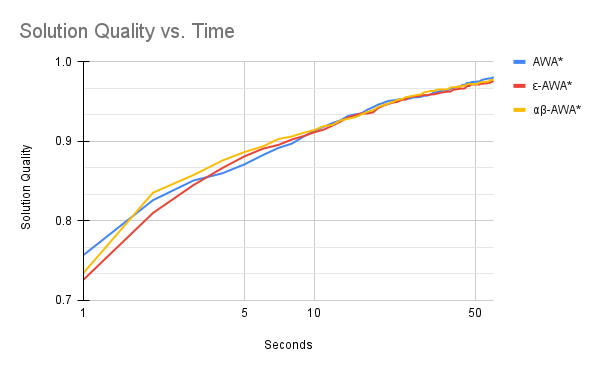
\includegraphics[width=\linewidth]{media/correct-Solution Quality vs. Time.png}
    \caption{Quality Convergence with Correct Tile Placement Heuristic.} \label{fig:conv-correct}
\end{figure}

While in the beginning AWA* actually has the best incumbent solutions, they all more or less approach the optimal solution at the same rate. This seems to simply demonstrate just how bad the Correct Placement heuristic is. I think what is going on here is that the Correct Placement heuristic is so bad it affectively adds and pulls nodes from the open list at random and so adding an exploration technique in no way helps since choosing the `best' node is also, basically, exploratory.

% \begin{figure*}
% 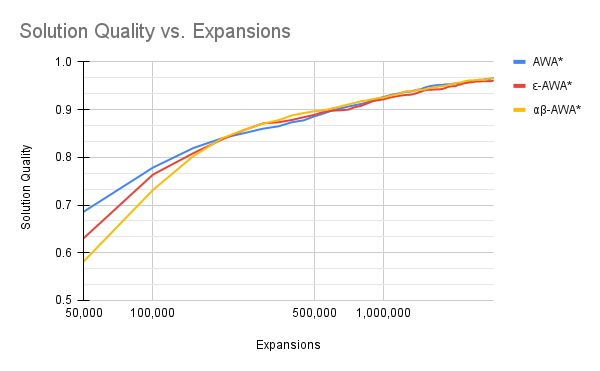
\includegraphics{media/correct-Solution Quality vs. Expansions.png}
% 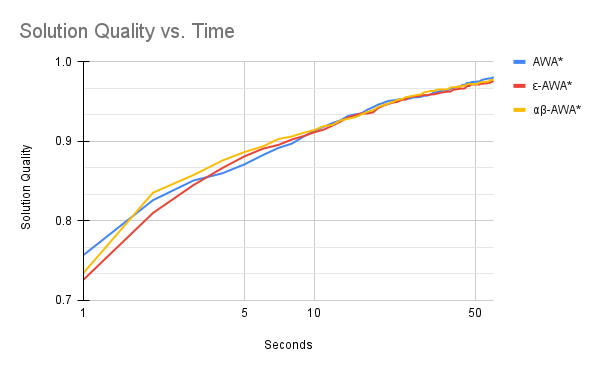
\includegraphics{media/correct-Solution Quality vs. Time.png}
% \caption{Quality Convergence with a Bad Heuristic.} \label{fig:conv-correct}
% \end{figure*}

